\subsection{Boosting Antenna Performance: The Magic of Terminating Resistors!}

\begin{tcolorbox}[colback=gray!10, colframe=black, title=E9C06] What is the effect of adding a terminating resistor to a rhombic or long-wire antenna?
\begin{enumerate}[label=\Alph*.]
    \item It reflects the standing waves on the antenna elements back to the transmitter
    \item \textbf{It changes the radiation pattern from bidirectional to unidirectional}
    \item It changes the radiation pattern from horizontal to vertical polarization
    \item It decreases the ground loss
\end{enumerate} \end{tcolorbox}

\subsubsection{Related Concepts}

To answer this question, it's important to understand the function of terminating resistors in antenna systems, particularly in rhombic and long-wire antennas. A terminating resistor is utilized at the open end of an antenna element to absorb radio frequency energy, thereby reducing reflected standing waves and altering the radiation pattern of the antenna.

\subsubsection{Understanding Antenna Radiation Patterns}

A long-wire antenna is typically bidirectional, radiating effectively in two opposite directions. When a terminating resistor is applied, it helps to change this pattern to a unidirectional radiation pattern. This means that the energy transmitted from the antenna is primarily radiated in one direction rather than back and forth.

\subsubsection{Antenna Theory}

1. \textbf{Standing Waves:}: When an antenna is not properly terminated, standing waves occur due to the reflection of signals. This can cause inefficiency in transmission and reception. 
2. \textbf{Radiation Pattern:}: The radiation pattern of an antenna describes how the antenna radiates energy into space. A bidirectional antenna radiates equally in two opposite directions, while a unidirectional antenna focuses energy in one direction.
3. \textbf{Ground Loss:}: Ground loss is the loss of power due to the absorption of energy by the ground. A terminating resistor does not directly affect ground loss; rather, it influences the overall efficiency and radiation pattern.

In summary, the addition of a terminating resistor allows for efficient utilization of the antenna, changing its characteristics to improve performance.

\subsubsection{Calculation Example}

If necessary, calculating the effect of the resistor on antenna impedance can be relevant. However, precise calculations depend on the specific parameters of the antenna. The input impedance of a long-wire antenna can be calculated using:

\[
Z_{in} = R + jX
\]

Where:
- \( R \) is the resistive component (often associated with radiation resistance)
- \( jX \) is the reactive component (indicating energy that is not radiated but rather stored and returned)

If you change the terminating impedance to a specific value \( Z_t \), it ideally should equal the radiation resistance for maximum power transfer without standing waves.

For example, if the radiation resistance is 75 Ohms and you add a terminating resistor of 75 Ohms, you would have:

\[
Z_{in} = 75 + j0 \, \text{Ohms}
\]

Having \( R \) matched with \( Z_t \) allows for efficient radiation in the designated direction.

\subsubsection{Illustration with TikZ}

\begin{center}
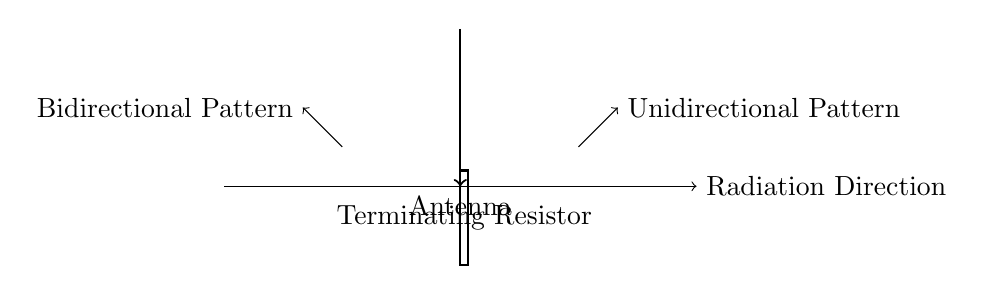
\begin{tikzpicture}
    \draw[->] (-3,0) -- (3,0) node[right] {Radiation Direction};
    \draw[->, thick] (0,2) -- (0,0) node[below] {Antenna} ;
    \draw[thick] (0,-1) rectangle (0.1,0.2) node[pos=.5] {Terminating Resistor};
    \draw[->] (1.5,0.5) -- (2,1) node[right] {Unidirectional Pattern};
    \draw[->] (-1.5,0.5) -- (-2,1) node[left] {Bidirectional Pattern};
\end{tikzpicture}
\end{center}
